\label{impl}
\section{Implementation}

\begin{figure*}
\centering
\begin{minipage}[b]{0.45\linewidth}
	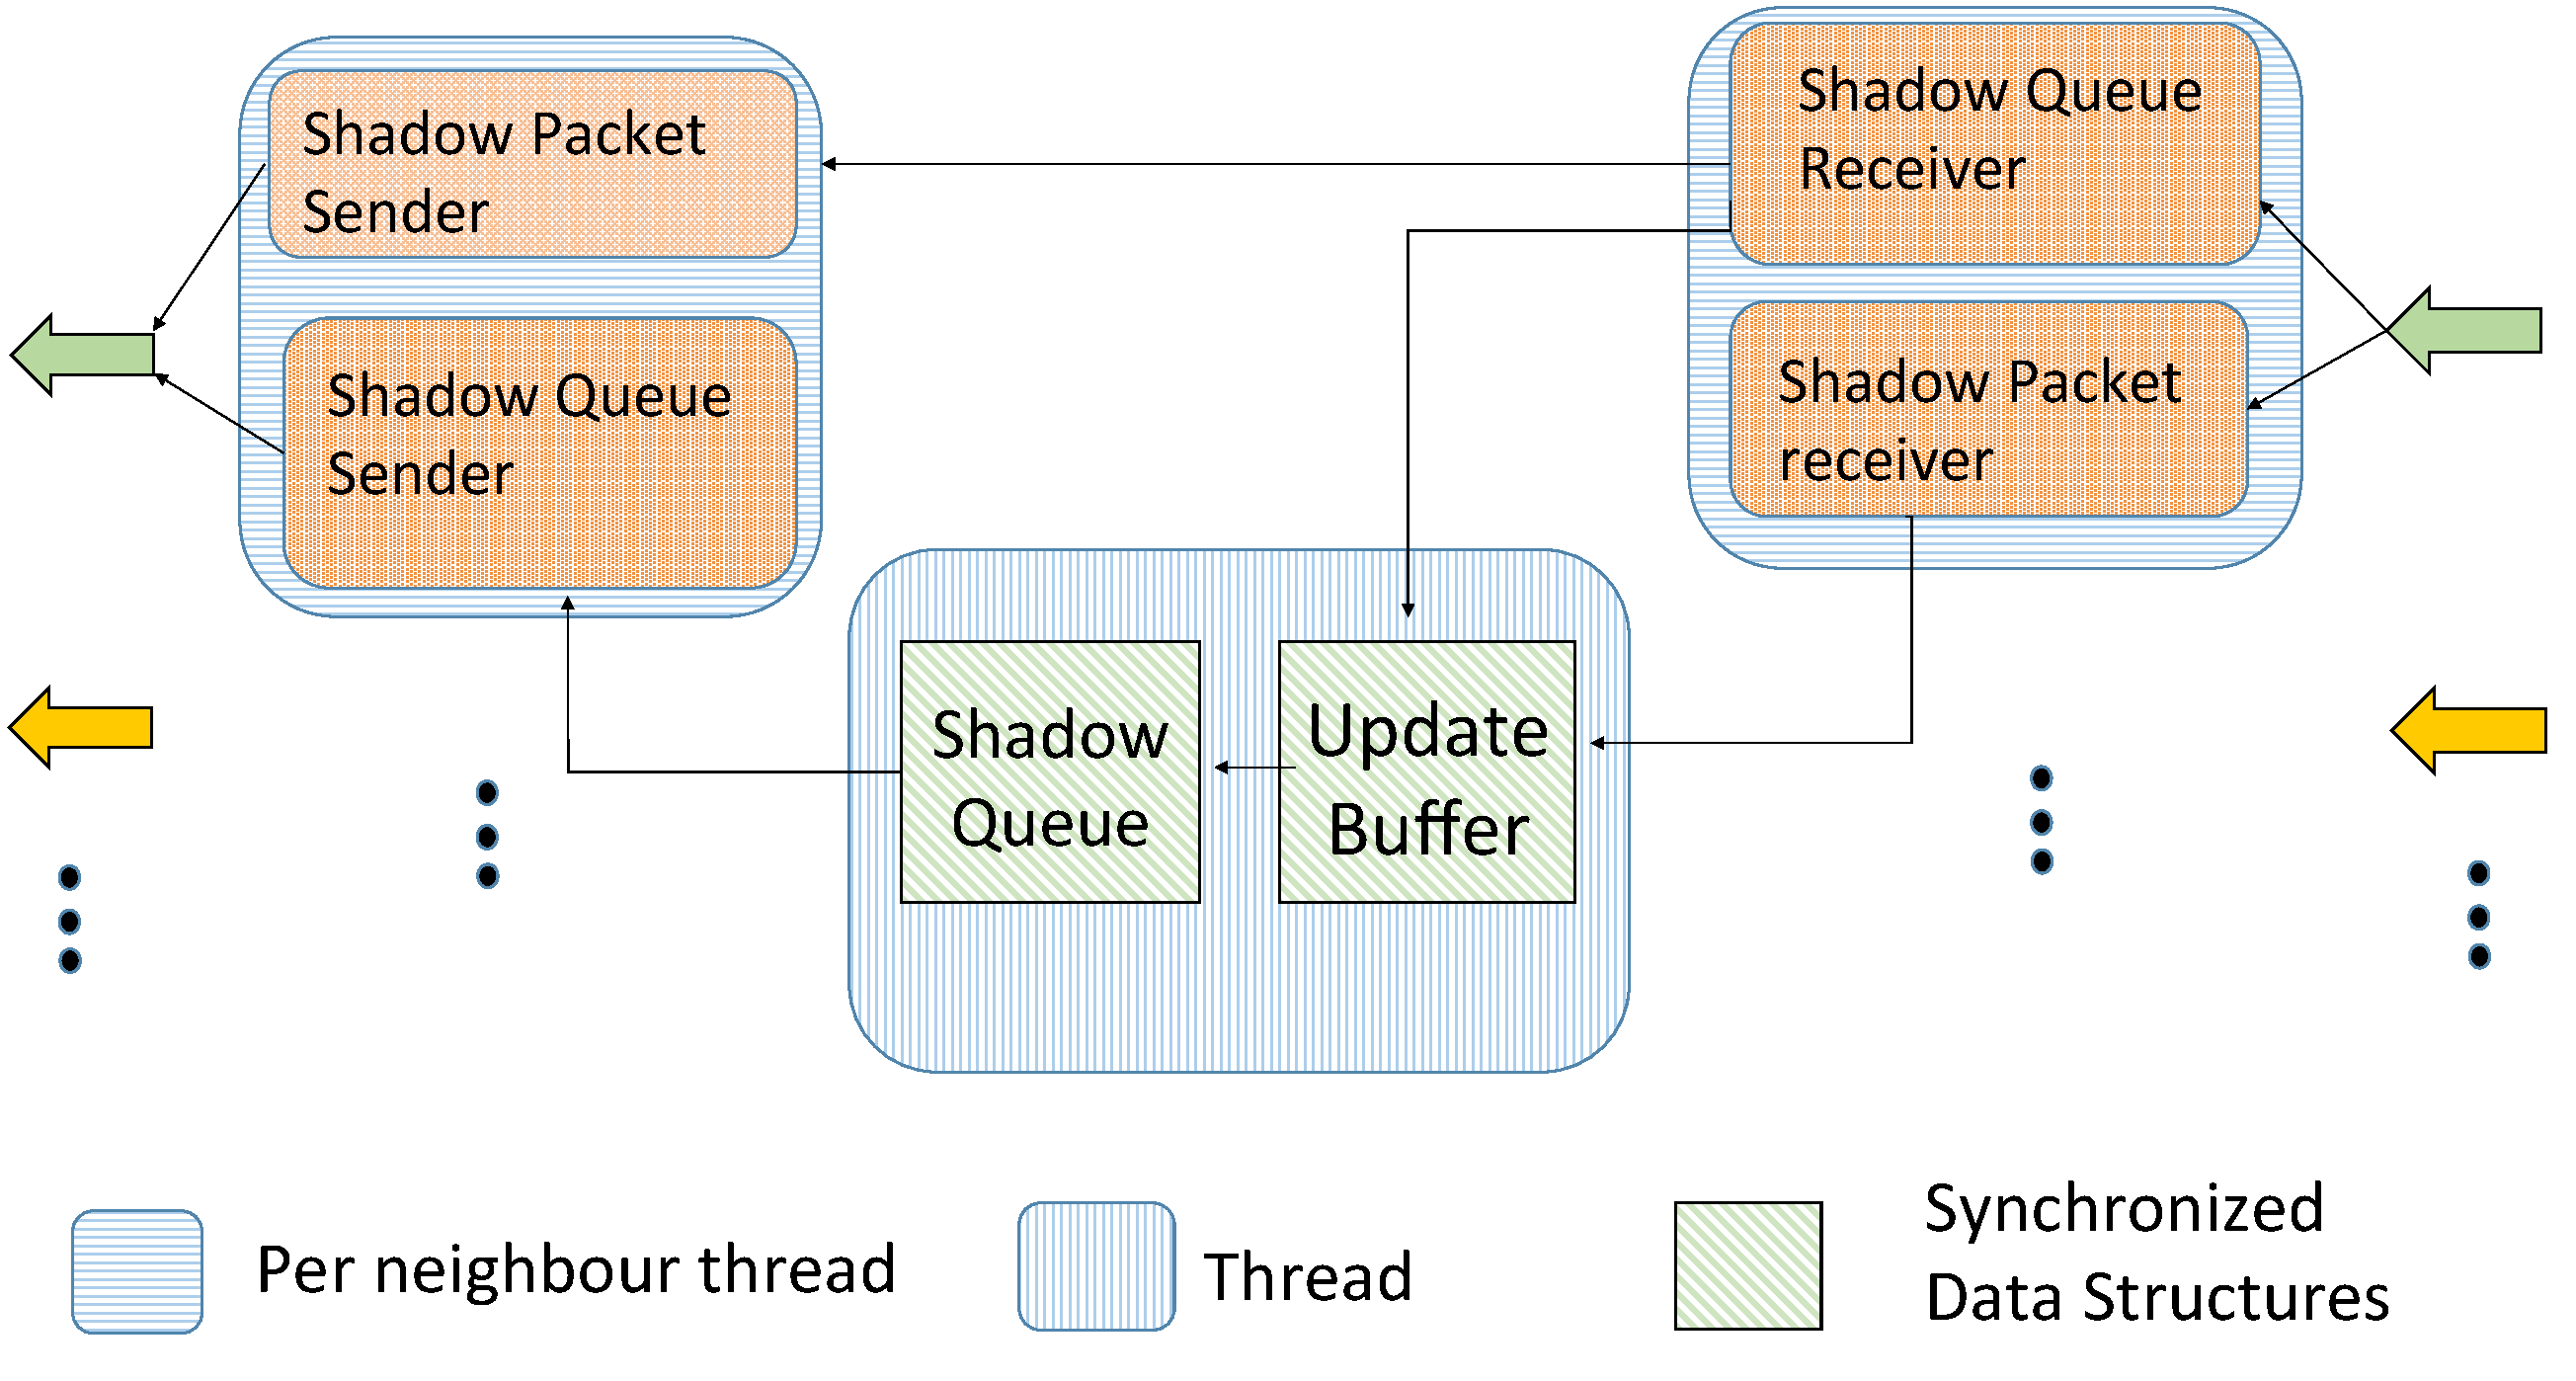
\includegraphics[width=2.4in]{./figures/controlpath2.pdf}
	\caption{Control path}
	\label{fig:control}
	\centering
	%\small Control path
\end{minipage}
\begin{minipage}[b]{0.45\linewidth}
	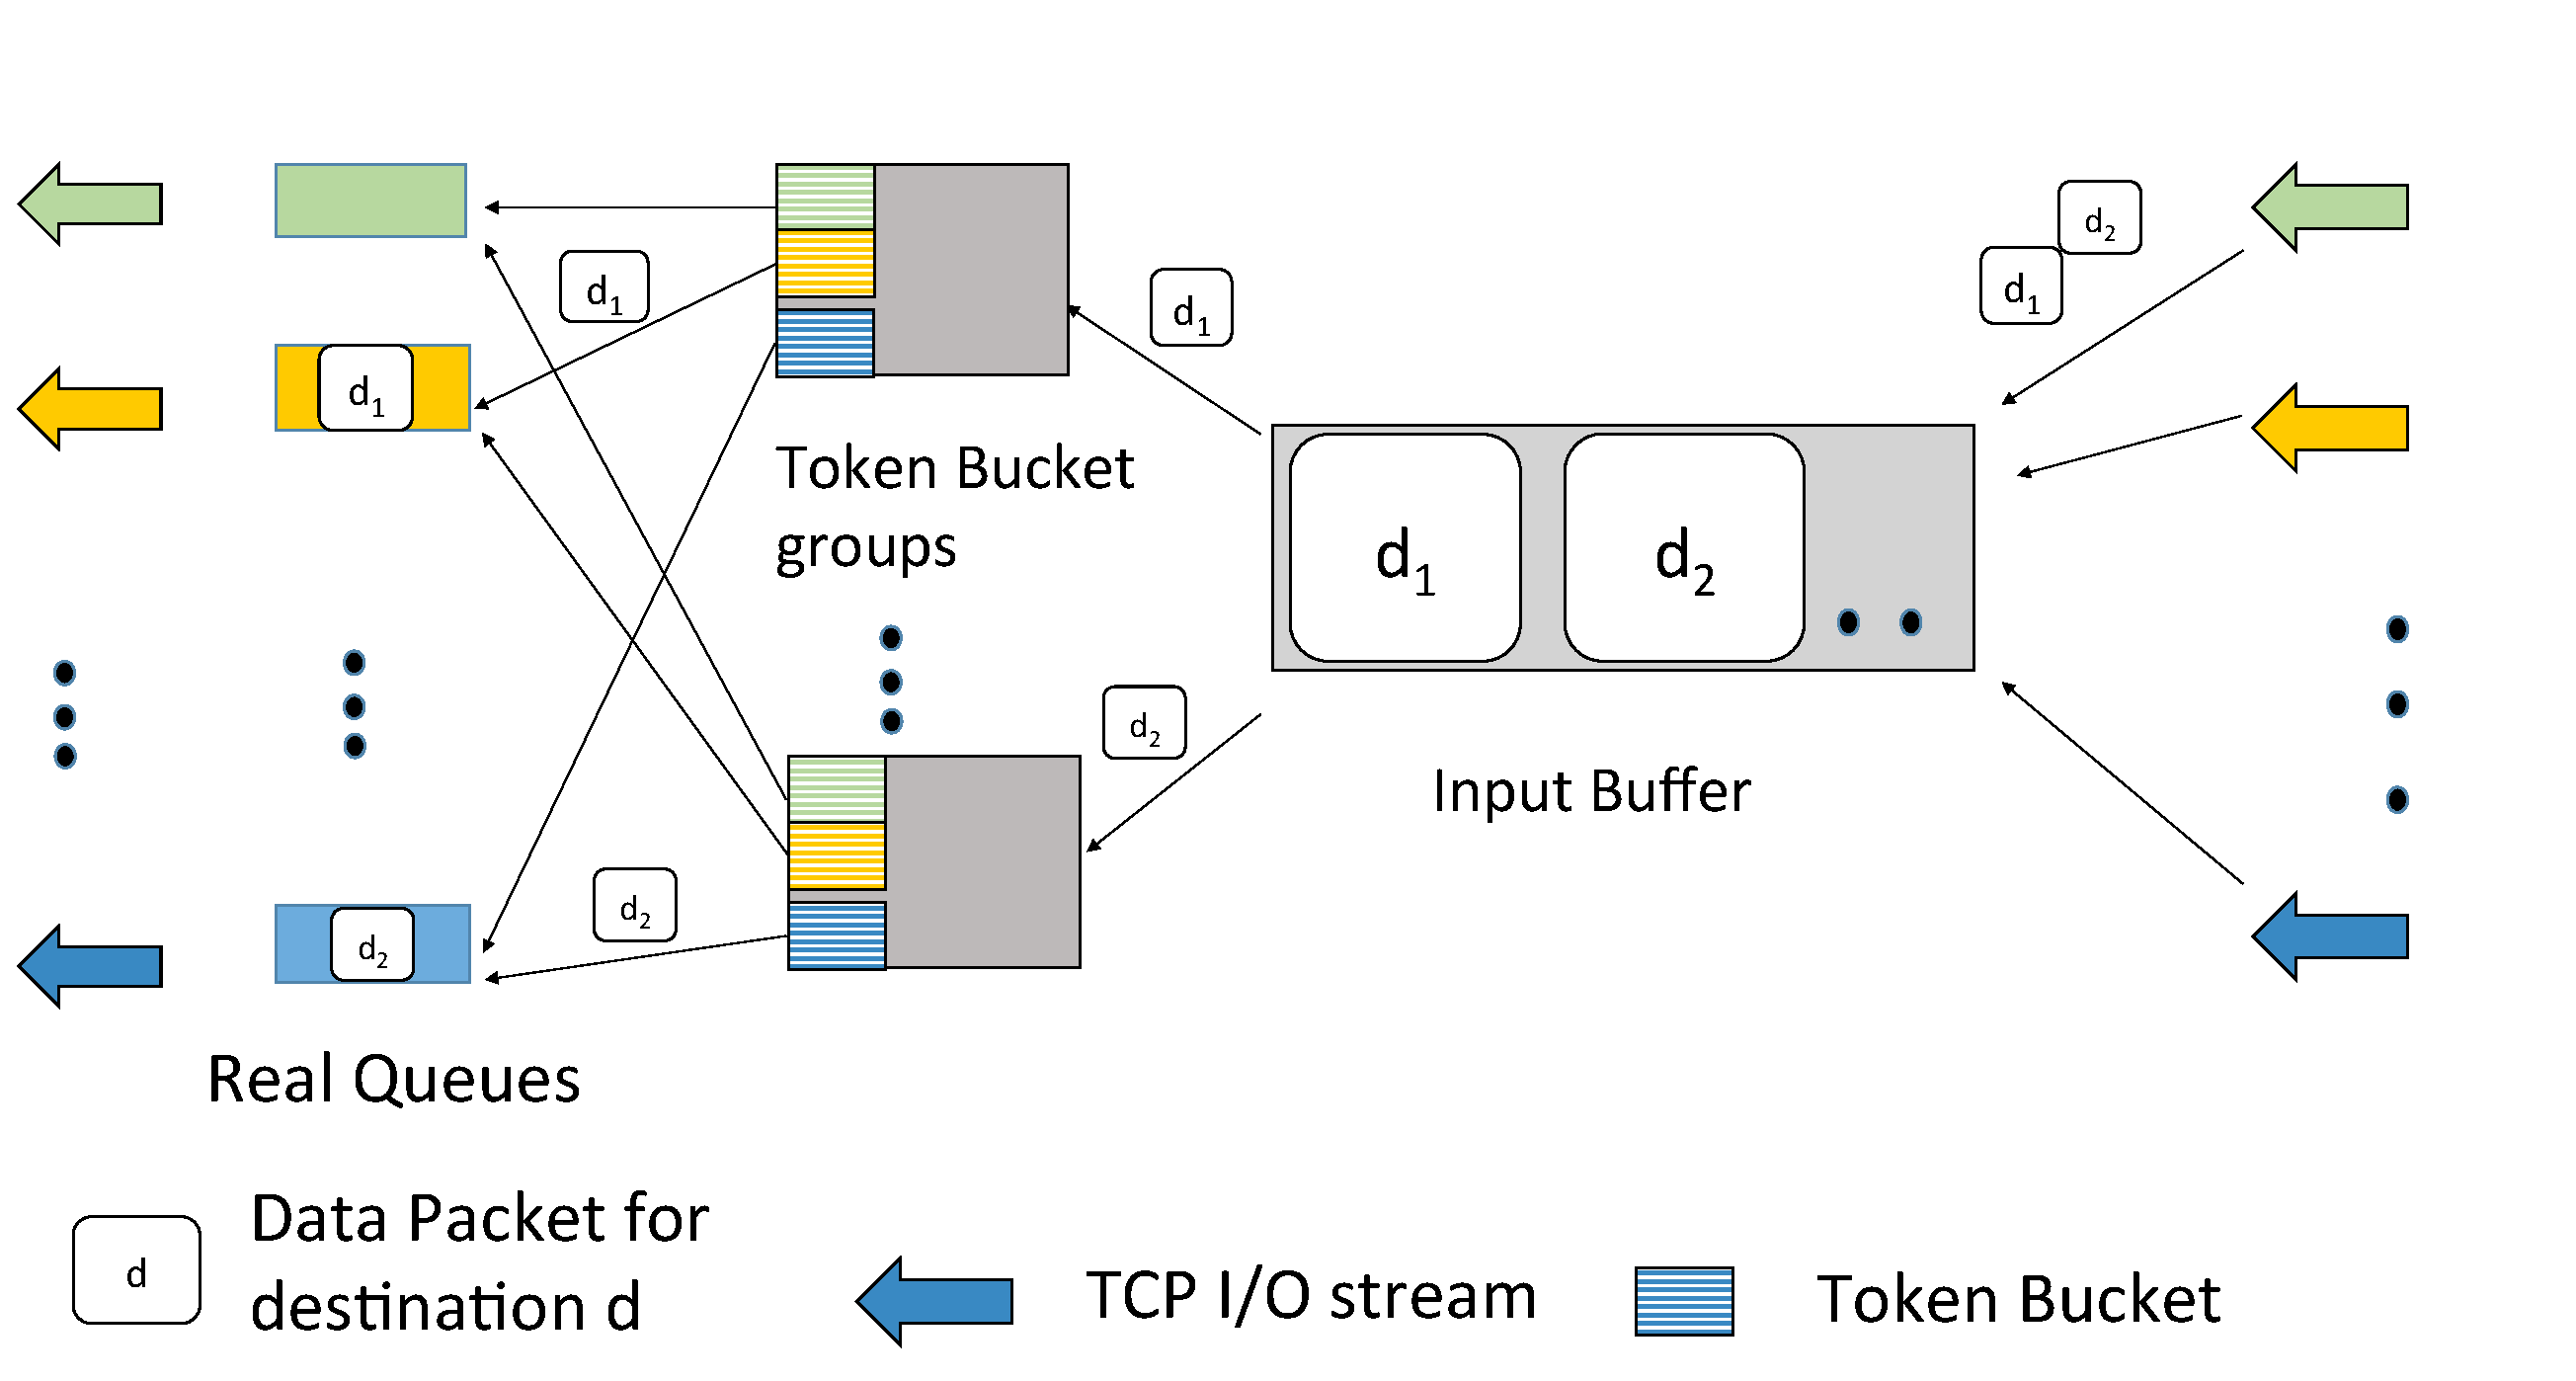
\includegraphics[width=2.4in]{./figures/datapath4.pdf}
	\caption{Data path}
	\label{fig:data} 
	\centering
	%\small Data path 
\end{minipage}
%\caption{\small Control path and data path in the real implementation}
%\label{fig:TCompare}
\end{figure*}


We implement the protocol as on overlay network over TCP/IP. We test the basic backpressure protocol as well as BP STEP-UP with different combinations of optimizations to identify the best one/combination. The rest of this section gives an overview of overlay node implementation. It consists of two parts - (a)Data Path which deals with routing and transmission of real packets from the FIFO queues and (b)Control Path which is responsible for transmission of shadow packets and exchange of information regarding shadow queues. 

\textbf{Data Path}(Figure~\ref{fig:data}) handles the routing and scheduling of Data packets. Each node maintains an incoming data channel per neighbor, each of which drains data packets into an \textit{input buffer} (FIFO queue) in a FIFO fashion. Packets from different channels may inter-mix in an arbitrary order depending on synchronization constructs of the \textit{input buffer}. Like incoming channels, outgoing data channels are maintained for each neighbor, each of which drains packets from corresponding \textit{real queue} in FIFO fashion. A system-wide thread transfers packets from \textit{input buffer} to an appropriate \textit{real queue} based on \textit{token buckets} ~\cite{Srikant3}. A \textit{token bucket group} is maintained for each destination, which contains \textit{token buckets} for each neighbor (or \textit{real queue}). A packet for destination \textit{d} goes to the smallest \textit{token bucket} in the corresponding group.

\textbf{Control Path} (Figure~\ref{fig:control}) describes the flow of control information i.e. number of shadow packets transferred and shadow queue length advertisements. Like data channels, incoming and outgoing control channels are maintained for each neighbor. Control information received from neighbors is buffered before it is applied to update nodes' own shadow queues. The way buffered updates are applied to shadow queues defines the synchronization construct. Waiting for updates from all the neighbors maps to slotted time assumption, which may result in high convergence time (since it is as slow as the slowest neighbor). The other extreme is to apply updates as soon as they are received, which is not proved to converge. We will test the system with different synchronization constructs. Note that updating shadow queue includes adjusting shadow queue lenghts, generating shadow packets (to be sent to neighbors) and updating token buckets, which determines the DataPath.
